\section{Problem analysis}

\subsection{Analysis of automata generated by approximate Kleenex}
To try to get an idea of what problems approximate Kleenex has, we tried to do
some visualization of the following simple program, and also
trying to manually generate the transducer to see if there was something it did
wrong.
\begin{center}
    \texttt{main := (/AT/<1> | ~/./)*}
\end{center}

Which translates to the following core Kleenex program,
\begin{align*}
    N0      &:= N1\ |\ N7\\
    N1      &:= N2-1\ |\ N6\\
    N2_0    &:= \texttt{A}\ N3_0\\
    N3_0    &:= \texttt{"A"}\ N4_0\\
    N4_0    &:= \texttt{T}\ N5_0\\
    N5_0    &:= \texttt{"T"}\ N0\\
    N2_1    &:= \texttt{A}\ N3_1\ |\ \texttt{.}\ N3_0\\
    N3_1    &:= \texttt{"A"}\ N4_1\\
    N4_1    &:= \texttt{T}\ N5_1\ |\ \texttt{.}\ N5_0\\
    N5_1    &:= \texttt{"T"}\ N0\\
    N6      &:= \texttt{.}\ N0\\
    N7      &:= \epsilon\\
\end{align*}
Figure \ref{fig:oft} and Figure \ref{fig:sst} repectively show the OFT and SST
of the program. So far we could see those two correspond correctly to the
program. Though it is possibly to improve the OFT by hand, as seen in Figure
\ref{fig:opt}, how this translates to the SST is a bit harder to see, as the
SST already only has 5 states, but the transition relation is quite complex,
and there are some transitions that could be merged. If these optimizations
could be generalized, they could probably help immensely on some of the program
sizes and performance, since from a random state out of $2556$ in our Ranges
pattern with $k = 1$ (which generated the longest C file) we see a single
transition executing 82 lines of C code to make the transition, and the state
overall being 650 lines long.

\begin{figure}[!hb]
  \centering
  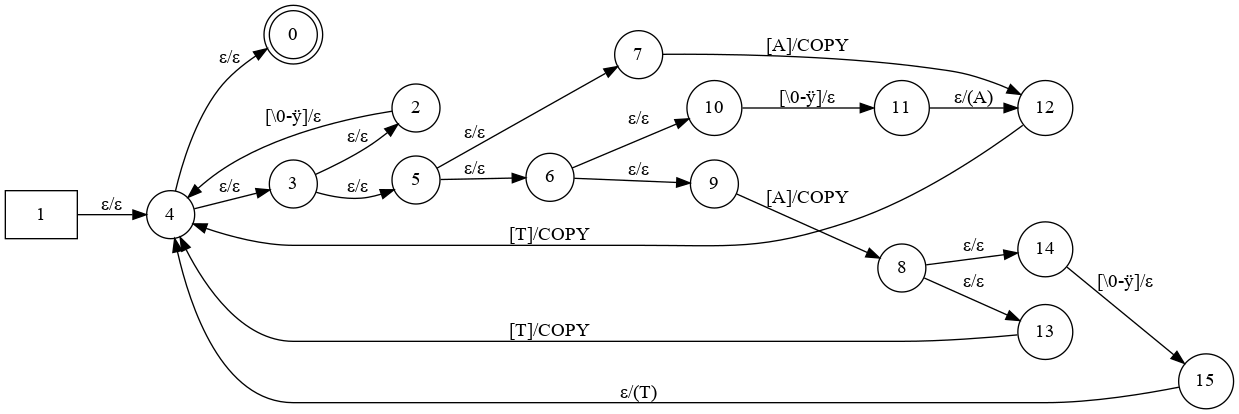
\includegraphics[width=0.9\textwidth]{images/oft.png}
  \caption{OFT of the simple approximate Kleenex program}
  \label{fig:oft}
\end{figure}
\begin{figure}[!hb]
  \centering
  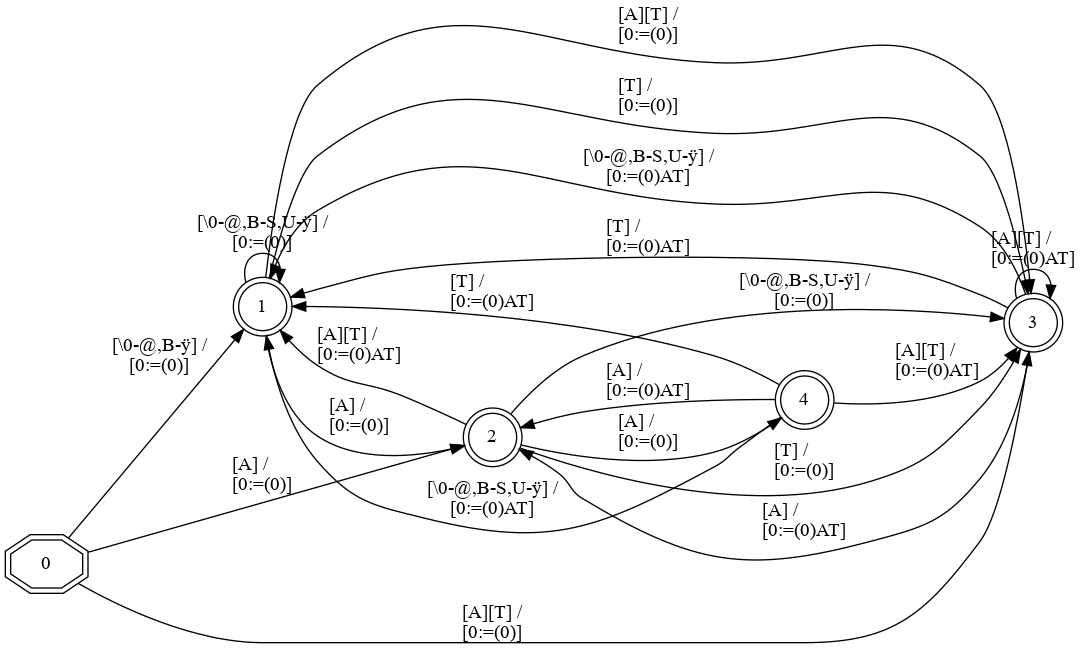
\includegraphics[width=0.9\textwidth]{images/sst.png}
  \caption{SST of the simple approximate Kleenex program}
  \label{fig:sst}
\end{figure}

\begin{figure}[!hb]
  \centering
  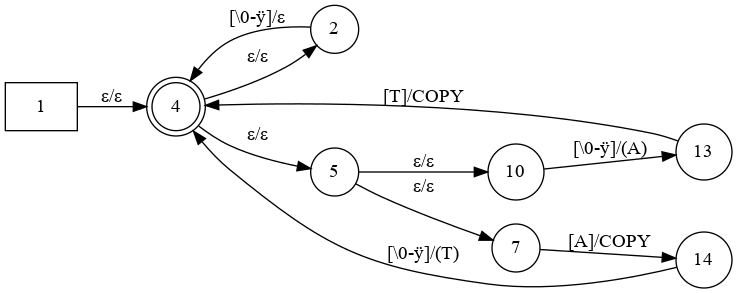
\includegraphics[width=0.9\textwidth]{images/opt.png}
  \caption{An optimized version of the OFT}
  \label{fig:opt}
\end{figure}

\subsection{Ideas for improving Kleenex}
% TODO: write properly

The result of the $k$-fold rewrite of a core Kleenex program, as described in
Troelsen's thesis~\cite{troelsen2016approximate} and exemplified in
Section~\ref{sec:approx-kleenex}, is proved in his thesis to be possible to
execute in time $\mathcal{O}(mnk)$ by determinization to an SST, where $n$ is
the size of the input string and $m$ is the size of the transition relation of
the corresponding NFST. This is proved by arguing that the growth of the number
of transitions in the transducer is in the order $\mathcal{O}(mk)$ (for $k>0$),
since the transformation adds $k$ new transitions to the transducer for each
existing transition and at most a constant number of additional transitions for
each of these new transitions, depending on the error metric. The
aforementioned time bound then follows from the result
in~\cite{grathwohl2016kleenex} that the SST can be implemented to execute in
time $\mathcal{O}(mn)$.

%This utilizes the results of Theorem 1 and Corollary 1 in the POPL paper.

Grathwohl et al.~\cite{grathwohl2016kleenex} also prove that for an NFST of
size $m$, i.e. with $m$ transitions, there is a semantically equivalent SST
with $\mathcal{O}(2^{m \log m})$ states. A corollary to this is that for a core
Kleenex program with a corresponding transducer of size $m$, allowing
approximate matches with up to $k$ errors, there is an SST with
$\mathcal{O}(2^{mk \log mk})$ states. Thus, the number of states in the SST
resulting from the rewriting of core Kleenex and following determinization of
the NFST, is exponential in $k$.

This seems to suggest a potential cause of the increased compilation times when
using approximate matching in Kleenex and the very large output programs that
it generates. Thus, one may be interested in exploring ways to avoid the
increase in size of the NFST.

% TODO: Talk about the inconvenient way that counting errors is represented by
% directly encoding it in the grammar rather than simply counting the errors.

% Theorem 2 from the POPL paper states that for an oracle machine of size $m$,
% i.e. the size of the transition relation, there is a (semantically equivalent)
% SST with $O(2^{m \log m})$ states.

% Counters, implemented as optimization in the implementation vs. updating the
% automata models.

\subsubsection{Tagged automata}

In his bachelor's thesis~\cite{enevoldsen2015pattern}, Sune Enevoldsen uses the
concept of a tagged automaton, based on work by Ville
Laurikari~\cite{laurikari2000nfas, laurikari2001efficient} and inspired by
Levenshtein automata~\cite{schulz2002fast}, to do approximate regular string
matching. This model was originally introduced to solve the problem of
extracting the position of matches for subexpressions of a regular expression,
however Laurikari also suggests its application to approximate matching.

A nondeterministic automaton with tagged transitions, or a tagged NFA, is a
finite automaton extended with a set of tags which may be set or modified on
each transition in the transition relation. The idea is to use these tags as
counters which keep track of the allowed number of errors, e.g. insertions,
deletion, and substitutions. A formal definition follows:

% Thus, the tagged automata for a given regular expression $RE$ will accept the
% strings in $\mathcal{L}(RE)$ as well as any string that is within a certain
% error distance of a string in $\mathcal{L}(RE)$.

\begin{definition}[NTA]
  A \emph{nondeterministic tagged automaton} (NTA) is a structure
  $(\Sigma, Q, q^s, F, T, t_0, \Delta)$, where $\Sigma$ is a finite alphabet,
  $Q$ is a finite set of states, $q^s$ is the initial state, and
  $F \subseteq Q$ is the set of final states. $T$ is a set of possible tag
  values, $t_0$ is the initial tag value and $\Delta$ is the transition
  relation
  \[
    \Delta \subseteq Q \times T \times \Sigma[\epsilon] \times Q \times T \;.
  \]
\end{definition}

The transition relation can also be described in terms of functions on tag
values. For each transition from state $p$ to state $q$ on input symbol $a$,
define a function $U_{p,a,q}$ from the set of tags $T$ to sets of tags. For the
purpose of approximate matching, and as in Enevoldsen's thesis, these functions
will always return just a singleton set or the empty set. Such a tag function
may ignore the tag, i.e. just return a singleton set of the given unchanged
tag, it may set a new tag independent of the current tag value, or it may set a
tag value depending on the current value. In particular, if
$U_{p,a,q}(t) = \emptyset$, then the automaton cannot transition from state $p$
to state $q$ on symbol $a$ when the tag $t$ is set.

We mark the transitions in the automaton with the tag functions, or just with
the new tag value if the function does not depend on its argument.

To use this automaton for approximate regular string matching using the
Levenshtein distance metric, we can set $T = \mathbb{N}^3$ and $t_0 =
[0,0,0]$. Thus, when entering a subexpression which allows a specified number
of substitutions, insertions, and deletions, the ingoing transition can set the
tag to the allowed errors. Similarly when leaving the subexpression, the tag
can be reset to $[0,0,0]$. For a mismatch, the tag function will be
\[
  M([m,i,d]) =
  \begin{cases}
    \emptyset     & \text{if } m = 0 \\
    \{[m-1,i,d]\} & \text{otherwise}
  \end{cases}
\]
and analogously for insertions, denoted $I$, and deletions, denoted $D$.

Thus, for Thompson's construction~\cite{thompson1968programming}, the case for
a literal character regular expression $a \in \Sigma$ is changed to the
following:

\begin{center}
\begin{tikzpicture}[->,>=stealth',shorten >=1pt,auto,node distance=2.0cm,
  semithick, main/.style={circle,draw,minimum width=10pt}]
    \node (q0) {};
    \node[main] (q1) [right = 5mm of q0] {};
    \node[main,accepting] (q2) [right = of q1] {};
    \path (q0) edge (q1)
    (q1) edge [loop above] node {$./I$}
    (q1) edge node {$a$} (q2)
    (q1) edge[bend left] node {$\epsilon/D$} (q2)
    (q1) edge[bend right] node[below] {$\bar{a}/M$} (q2);
\end{tikzpicture}
\end{center}

For the sake of simplicity, consider now just the mismatch error type. Extend
the notion of tagged automata to transducers in the straightforward way,
e.g. by added the output alphabet to the tagged automaton and modifying the
transition relation to include output, as follows:
\[
  \Delta \subseteq Q \times T \times \Sigma[\epsilon] \times \Gamma[\epsilon]
  \times Q \times T
\]

One could transform an NFST for exact matching to a tagged NFST by translating
the core Kleenex term $N ::= \mathtt{a}N'$ to the following transitions in the
NFST:

\begin{center}
  \begin{tikzpicture}[->,>=stealth',shorten >=1pt,auto,semithick,
    main/.style={minimum width=10pt}]
    \node (q0) {$N$};
    \node (q0a) [above right = 2mm and 10mm of q0] {$N_0$};
    \node (q0b) [below right = 2mm and 10mm of q0] {$N_1$};
    \node (q1) [below right = 2mm and 10mm of q0a] {$N'$};
    \path (q0) edge node {$\epsilon_0/\epsilon$} (q0a)
    (q0) edge node [below left] {$\epsilon_1/\epsilon$} (q0b)
    (q0a) edge node {$\mathtt{a} / \epsilon$} (q1)
    (q0b) edge node [below right] {$\bar{\mathtt{a}}/\epsilon, M$} (q1);
  \end{tikzpicture}
\end{center}

Here the $M$ in $\bar{\mathtt{a}}/\epsilon, M$ denotes the tag function on the
transition, which decrements the number of allowed mismatches by one.

Continuing the example from Section~\ref{sec:approx-kleenex}, a tagged
transducer for the described core Kleenex program, accepting the language $a^*$
with a given number of allowed substitutions, may be realized as shown in
Figure~\ref{fig:tagged-transducer}.

\begin{figure}[!hb]
  \centering
  \begin{tikzpicture}[>=stealth',semithick,scale=0.14]
  \tikzstyle{every node}+=[inner sep=0pt,minimum width=10pt]
  \draw [black] (26.3,-22.6) circle (3);
  \draw (26.3,-22.6) node {$N$};
  \draw [black] (44.6,-15.4) circle (3);
  \draw (44.6,-15.4) node {$N_\epsilon$};
  \draw [black] (59.5,-15.4) circle (3);
  \draw (59.5,-15.4) node {$q_f$};
  \draw [black] (59.5,-15.4) circle (2.4);
  \draw [black] (59.5,-27.2) circle (3);
  \draw (59.5,-27.2) node {$N_A$};
  \draw [black] (38.8,-38.7) circle (3);
  \draw (38.8,-38.7) node {$N''_A$};
  \draw [black] (40.4,-31.1) circle (3);
  \draw (40.4,-31.1) node {$N'_A$};
  \draw [black] (47.6,-15.4) -- (56.5,-15.4);
  \fill [black] (56.5,-15.4) -- (55.7,-14.9) -- (55.7,-15.9);
  \draw (52.05,-14.9) node [above] {$\epsilon$};
  \draw [black] (29.09,-21.5) -- (41.81,-16.5);
  \fill [black] (41.81,-16.5) -- (40.88,-16.33) -- (41.25,-17.26);
  \draw (34.12,-18.47) node [above] {$\epsilon_1$};
  \draw [black] (29.27,-23.01) -- (56.53,-26.79);
  \fill [black] (56.53,-26.79) -- (55.8,-26.18) -- (55.67,-27.17);
  \draw (43.36,-24.27) node [above] {$\epsilon_0$};
  \draw [black] (57.844,-29.699) arc (-37.28549:-84.6053:22.872);
  \fill [black] (41.8,-38.61) -- (42.64,-39.04) -- (42.55,-38.04);
  \draw (52.15,-36.34) node [below] {$\epsilon_1$};
  \draw [black] (56.695,-28.262) arc (-70.92823:-85.99078:51.775);
  \fill [black] (43.4,-30.98) -- (44.23,-31.42) -- (44.16,-30.42);
  \draw (50.94,-30.68) node [below] {$\epsilon_0$};
  \draw [black] (35.963,-37.737) arc (-114.02842:-170.32022:16.304);
  \fill [black] (26.53,-25.59) -- (26.17,-26.46) -- (27.16,-26.29);
  \draw (29.16,-34.26) node [left] {$./\epsilon,M$};
  \draw [black] (37.549,-30.17) arc (-110.92075:-131.24549:30.097);
  \fill [black] (28.45,-24.69) -- (28.73,-25.59) -- (29.38,-24.84);
  \draw (30.81,-28.33) node [below] {$a/\epsilon$};
  \draw [black] (20,-22.6) -- (23.3,-22.6);
  \fill [black] (23.3,-22.6) -- (22.5,-22.1) -- (22.5,-23.1);
  \end{tikzpicture}
  \caption{Conceptual visualization of a tagged transducer for core Kleenex
    programmed described and rewritten in Section~\ref{sec:approx-kleenex}.}
  \label{fig:tagged-transducer}
\end{figure}

Compare this to the transducer for the rewritten core Kleenex program, shown in
Appendix~\ref{app:approx-kleenex-example}. Furthermore, this tagged transducer
is of a fixed size independent of $k$, compared to the linear growth of the
rewritten program.

It may be possible to simulate a tagged transducer like a regular transducer,
using path-tree simulation, by extending the state of each leaf of the path
tree to include the number of allowed mismatches in that state. A leaf in the
path tree will then be able to step on a given input symbol according to the
transition relation, if the tag function maps the current tag to a nonempty
set, the single element of which will then be the new tag, otherwise the path
will fail.

The question still remains, whether it is possible to determinize such an
automaton to an SST and how many states it would generate. Following the
argument in \cite{soholm2015ordered}, there is a finite number of reduced path
trees, ignoring outputs, and since the value of $k$ for any given leaf is also
bounded, there is also a finite number of reduced path trees with associated
error counts. Thus, it should be possible to determinize these into a streaming
string transducer, that is, a deterministic automaton with abstract states
corresponding to the reduced path trees as states, transitions representing the
changes to the path tree during simulation, and registers storing the outputs
associated with each node in the path tree. The size of such an SST will have
to be investigated in future work.


\subsubsection{Scanning for subpatterns}

Another potential idea for improving the performance of approximate Kleenex is
to select subpatterns to search for, as also used in NR-grep and discussed
in~\cite{navarro2001nr}. Specifically for approximate Kleenex, where the size
of the SST appears to be a critical issue, compiling only a shorter and perhaps
simpler subpattern to an SST could significantly reduce the determinization
overhead. A good choice for a subpattern may be significantly simpler, yet its
occurrence in the text could yield a high probability for an actual match of
the whole pattern, depending on the assumptions made about the text. This
potential match can then be verified, e.g. by simulating the transducer using
path-tree simulation.

For example, consider the Kleenex program for the ranges benchmark case:
\texttt{(/[ACGT]/\{5,15\} /TGCAAGCGTTAAT/)<$k$>}, which could only be compiled
for $k\leq1$. Compiling only the pattern \texttt{/TGCAAGCGTTAAT/}, with errors
allowed, will significantly reduce the size of the SST, but is expected to
still provide a good indication for the probability of a match

As mentioned NR-grep, among others, uses this techniques and
\cite{navarro2001nr} describes techniques for selecting an optimal subpattern
under some simplifying assumptions about the text characters.

%%% Local Variables:
%%% mode: latex
%%% TeX-master: "main"
%%% End:
